% Fig. 1 -- teaser (figure*, top of page 1 or 2)
\begin{figure*}[tbp]
  \centering
  \subcaptionbox{Where exact repeats live (potential tier)\label{fig:scope}}{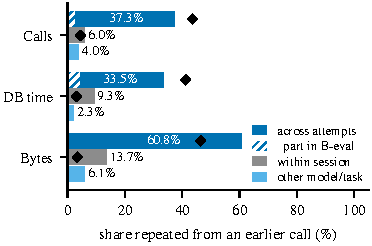
\includegraphics[height=1.62in]{figures/fig1a_scope}}\hfill
  \subcaptionbox{Reuse grows with $N$ (potential tier)\label{fig:ncurve}}{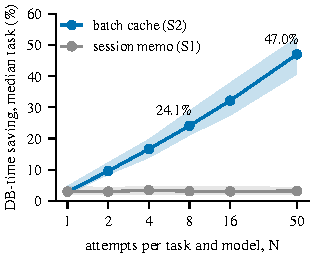
\includegraphics[height=1.62in]{figures/fig1b_ncurve}}\hfill
  \subcaptionbox{What each admission tier admits\label{fig:tiers}}{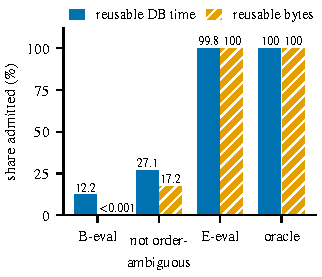
\includegraphics[height=1.62in]{figures/fig1c_tiers}}
  \caption{Where the database work of repeated agent runs repeats, and how much of it each admission tier can reuse
  on DAB. (a) Shares of calls, isolated DB-execution time and payload
  bytes among the 70,173 oracle-admitted calls, by the scope of the earlier exact repeat. The scopes are another
  attempt of the same task and model, the same session, and another model's or task's runs. Shares are pooled over 200
  random attempt orders. Diamonds mark the median task, and hatching marks the part in the B-eval subset. (b)
  Median-task saving of isolated DB-execution time in an unbounded, oracle-gated simulation with 200 resamples. S1 is
  a per-session cache, and S2 is a cache shared by a batch of $N$ attempts of one model on one task. Bands show the
  task-bootstrap 95\% CI, and $N=50$ uses the 268 of 270 task--model cells with 50 runs. (c) Share of the
  cross-attempt reusable DB time and bytes in the B-eval (certified), E-eval (assumption-based) and oracle (potential)
  subsets. The bar ``not order-ambiguous'' covers all calls except the successful ones with at least two distinct rows
  and no top-level \texttt{ORDER BY}. It is a conservative upper bound for any rule that guarantees serialized bytes across query plans in engine row order.}
  \label{fig:teaser}
  \Description{Three panels. Left: horizontal bars showing that repeats across attempts carry 37.3, 33.5 and 60.8 percent of calls, DB time and bytes, against 6.0, 9.3 and 13.7 percent within a session. Middle: lines showing the batch cache saving rising from 3 to 47 percent of DB time as attempts grow from 1 to 50 while the session cache stays near 3 percent. Right: bars showing the B-eval subset holds 12.2 percent of reusable DB time and almost no bytes, the calls that are not order-ambiguous 27.1 percent of the time and 17.2 percent of the bytes, while the E-eval subset and the oracle admit nearly all.}
\end{figure*}
